\chapter{Ray Optics} \label{ch:RayOps}
To understand heat loss characteristic of coupled LFR and TCR system more accurately, heat flux received by individual pipes inside TCR become an important information. Until now, most of studies performed on TCR assumes that all the pipes inside TCR are at uniform temperature {\bf give reference}. Present study is oriented towards examining this assumption of uniform temperature of pipes. For calculation of heat flux received by individual pipes in TCR, ray tracing calculation is required. For ray tracing study two methods were considered- Monte Carlo ray tracing (MCRT) and deterministic ray tracing. Given that the model under present study is 2-D and and geometry is quite simple. There was not any significant advantage of MCRT. Thus present study includes deterministic ray tracing for ray optics calculation. 
\section{Problem Statement}
The LFR system in the present study contains 8 parallel reflectors of width 1.8 m each for the entire length of reflection which can be seen in the fig. \ref{lfrsetup} and description can seen in the table \ref{lfrspectab}


\begin{figure}[H]
\begin{center}
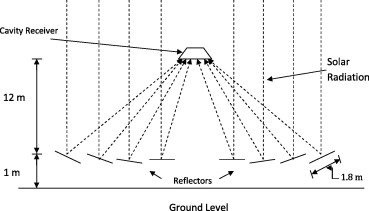
\includegraphics[width=0.65\textwidth]{lfrsetup.jpg}
\caption{LFR collector setup}
\end{center}
\label{lfrsetup}
\end{figure}


\begin{table}[H]
\centering
\caption{LFR specification}
\label{lfrspectab}
\begin{tabular}{@{}|l|c|@{}}
\toprule
\textbf{Items}                      & \textbf{Dimensions} \\ \midrule
Bottom width of the cavity          & 500 mm              \\ \midrule
Top width of the cavity             & 300 mm              \\ \midrule
Side length of the cavity           & 141 mm              \\ \midrule
Depth of the cavity                 & 100 mm              \\ \midrule
No of tubes in the cavity           & 8                   \\ \midrule
Absorber tube inner diameter        & 26.7 mm             \\ \midrule
Absorber tube outer diameter        & 33.4 mm             \\ \midrule
Absorber length                     & 384 m               \\ \midrule
No of reflector reflectors             & 8                   \\ \midrule
Reflector width                     & 1.8 m               \\ \midrule
Positions of reflectors from ground & 1 m                 \\ \midrule
Positions of cavity from the ground & 13 m                \\ \midrule
Gap between reflectors                  & 0.5 m                   \\ \midrule
Radius of  curvature (left to right) & 30 29 26 24 24 26 29 30 \\ \midrule
Optical efficiency                   & 80\%                    \\ \bottomrule
\end{tabular}
\end{table}
It is equipped with 1-D tracking.
\section{Focal point selection}
At first ray tracing was performed by keeping focal point of all the 8 reflectors at the center of the cavity. But as a result only 4 tubes at the center of the cavity receive the heat flux and 2 tubes in the center receive majority of the  heat flux which can be seen in the fig. \ref{rayTracingTCR_at_ope_focal_point}  So, before moving further single focal point notion was abandoned and distributed focal point options were explored. Since, in the problem statement there are 8 tubes as well as 8 reflectors, each reflector was assigned one tube as its focal point. This was done specially to distribute heat flux uniformly on the tubes. This is important because such LFR systems are used for heating working fluid for industrial purposes. They have requirement of certain fixed temperature for their task. Now, it is important to ensure that output temperature of the working fluid is roughly same (within few degree celsius) for all the tubes. To achieve that it becomes important to distribute heat flux uniformly on tubes. In this case, it was achieved by assigning one to one relationship between pipes and reflectors. Focal point of reflector was kept at the center of the pipe. By doing this it was ensured that heat flux is not received by the pipe at a single point but by certain length along its perimeter. By doing so relatively uniform heat flux was obtained on the pipes which can be seen in the fig. \ref{rayTracingTCR}

\begin{figure}[H]
\begin{center}
  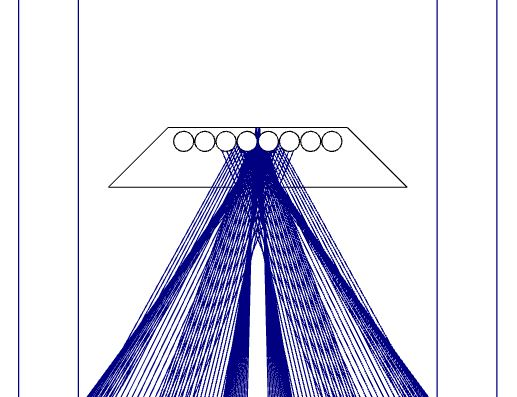
\includegraphics[width=0.65\textwidth]{rayTracingTCR_at_ope_focal_point.JPG}
\caption{Ray Tracing with focus on the center of the cavity}
\end{center}
\label{rayTracingTCR_at_ope_focal_point}
\end{figure}

\section{Ray optics simulation}\label{sec:rayopsim}
Ray optics simulation is performed in COMSOL Multiphysics 5.3 using ray optics module. Solar rays were assumed to be parallel. Sun has been modeled as a grid source. Since 2-D geometry is under study. Aforementioned grid is a linear grid of points from which parallel rays are generated. This linear grid is chosen wide enough so that all the reflectors are hit by incident rays. Absorption coefficient of the reflectors are defined to be 0.2 to take optical efficiency of the reflector system into account which is 80\% and can be seen in the table \ref{lfrspectab}. Incident rays after reflected by reflectors goes inside the trapezoidal cavity receiver. Glass at the bottom of trapezoidal cavity receiver is assumed to be fully transparent. Top, left and right sides of the cavity are set at wall condition of specular reflection with absorption coefficient of 0.1. Tubes inside the trapezoidal cavity receiver is set to absorb all rays falling on it. Deposited ray power is being calculated on all the tubes as well as top, left and right walls of the cavity which will be used further in the heat transfer simulation. Result obtained from this simulation can be seen in the fig. \ref{rayTracingTCR}

\begin{figure}[H]
\begin{center}
  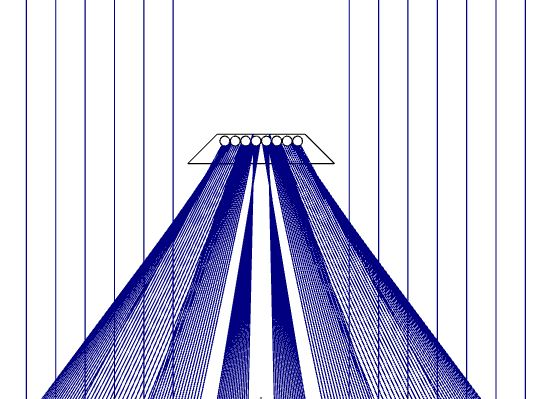
\includegraphics[width=0.65\textwidth]{rayTracingTCR.JPG}
\caption{Ray Tracing with distributed focus}
\end{center}
\label{rayTracingTCR}
\end{figure}

\subsection{Calculation of heat received by pipes: detailed description}\label{subsec:calcHeatRecPipesDetailedDescrip}
This subsection is dedicated for describing how calculation was done for determining amount of heat absorbed by each individual pipes after the simulation. Here explanation has been given for the case when rays are coming perpendicular to the earth's surface (local noon). For other cases same procedure has been followed. Since it is a 2-D study, unit of heat is given as W/m and unit of area is given as m. Please bear that in mind while moving further. As described in section \ref{sec:rayopsim} rays were launched by a linear grid source. Power of this source was kept to be 1 W/m. After simulation heat absorbed by all the pipes and cavity walls are provided by the software. However these values obtained from the software are for the case when source power is 1 W/m. In reality calculation are performed using heat flux. For heat transfer study which is the next part, one of the input parameters is solar flux at a given time say $I_{0}$ $W/m^2$. While ray optics simulation has been performed using input of heat not the heat flux. To overcome this problem following approach has been taken-
\begin{enumerate}
\item Obtain absorbed heat by each surface (pipes and walls) for 1 W/m source using software.
\item Since all the rays reflected by reflectors are going inside the cavity and all the rays going inside the cavity are fully absorbed, heat sent by reflectors is nothing but sum of total heat received by different surfaces inside the cavity in this case it is 0.598 W.
\item Heat absorbed by all the surfaces are divided by the sum of all the heat going inside the cavity (which is total heat reflected by the reflectors). By doing so, fraction of heat received by all the surfaces of total heat sent by the reflector is known for each surface.
\item Now, if for heat transfer simulation let's say available solar heat flux is $I_{0}\; W/m^2$. This is multiplied with the absorber area which is in this case 8 reflectors of width 1.8 m each so, 
\\
$ area = 8 * 1.8 m= 14.4 m$ \\
$ heat \:received\:by\:reflectors = I_{0}\; W/m^2 * 14.4 m = 14.4I_{0}\;W/m$  
\\
Since optical efficiency of reflectors is 80 \%, only 80 \% of received heat will be reflected to the cavity \\
$heat\: reflected = heat\: received * 80 \% = 11.52I_{0}\;W/m$ \\
\item Now that total reflected heat has been calculated and fraction of reflected heat received by each surface is already known. Heat received by each surface is calculated when solar flux is $I_{0}\;W/m^2$.
\end{enumerate}
 


This is the approach followed after each ray optics simulation and before heat transfer simulation. Heat received by each surface as calculated in step 5 is given as input for heat transfer simulation.

\section{Solar flux calculation}
Calculation of solar flux has been done for 31\textsuperscript{st} May at five different times over the day- 08:00, 10:00, 12:00, 14:00 and 16:00. It has been calculated over mumbai. Calculation parameters are given in the table \ref{tab:solarFluxCalcParams}.


\begin{table}[H]
\centering
\caption{Solar flux calculation parameters}
\label{tab:solarFluxCalcParams}
\begin{tabular}{@{}|c|c|@{}}
\toprule
\textbf{Parameters} & \textbf{Value} \\ \midrule
Location            & Mumbai         \\ \midrule
Lattitude           & 19.076         \\ \midrule
Longitude           & 72.88          \\ \midrule
Date                & 31st May       \\ \midrule
Inclination angle   & 0              \\ \bottomrule
\end{tabular}
\end{table}

For given day of the year hour angle has been calculated as function of local time. In this case for 31\textsuperscript{st} May\\ 
\[
n = 151 \qquad \qquad \text{where n = 1 for January 1\textsuperscript{st}} 
\]
Equation of time,
\begin{equation}
E_{t} =  9.87\times sin(2B)-7.53\times cos(B)-1.5\times sin(B)
\end{equation}
where, 
\[
B = \frac{360}{364}\big(n-81\big)
\]

Time correction factor,
\begin{equation}
TCF = 4\times (longitude - LSTM) + E_{t}
\end{equation}

Local standard time,
\begin{equation}
LST = Local\; time + \frac{TCF}{60}
\end{equation}
\begin{equation}\label{eq:hourAngle}
\omega = 15^0 (LST-12)
\end{equation}

Using equation \ref{eq:hourAngle} hour angle has been calculated which is further used in calculation of angle between solar rays and surface normal.

\begin{multline}
cos(\theta) = sin(\phi)*(sin(\delta)*cos(\beta)-cos(\delta)*cos(\omega)*sin(\beta))+\\
cos(\phi)*(cos(\delta)*cos(\omega)*cos(\beta)-sin(\delta)*sin(\beta))+ \\
cos(\delta)*sin(\omega)*sin(\beta)
\end{multline}

Solar heat flux,
\begin{equation}\label{eq:solarfluxcalc}
I_{0} = DNI\times cos(\theta)
\end{equation}

Using equation \ref{eq:solarfluxcalc} solar flux falling over reflectors is calculated  for different time of the day. By determining solar flux, heat received by pipes and other surfaces has been obtained as explained in subsection \ref{subsec:calcHeatRecPipesDetailedDescrip}. And then analysis of heat loss in trapezoidal cavity receiver has been performed in chapter \ref{ch_Heat_Transfer}.











